\subsection{Ruby on Rails}
\label{tag:rails}
本研究で提案したネットワークシミュレータは、Ruby on Railsを用いて実装されている。Ruby on Railsとは、Rubyで構築された、Webアプリケーションを開発するためのフレームワークである。特徴としてMVCアーキテクチャの採用や設定より規約という設計哲学などが挙げられる。
 MVCとは「Model」「View」「Controller」の頭文字であり、MVCアーキテクチャとはアプリケーションの構成が以下の図\ref{fig:MVC}のようになることに由来している。

\begin{figure}[htbp]
  \begin{center}
    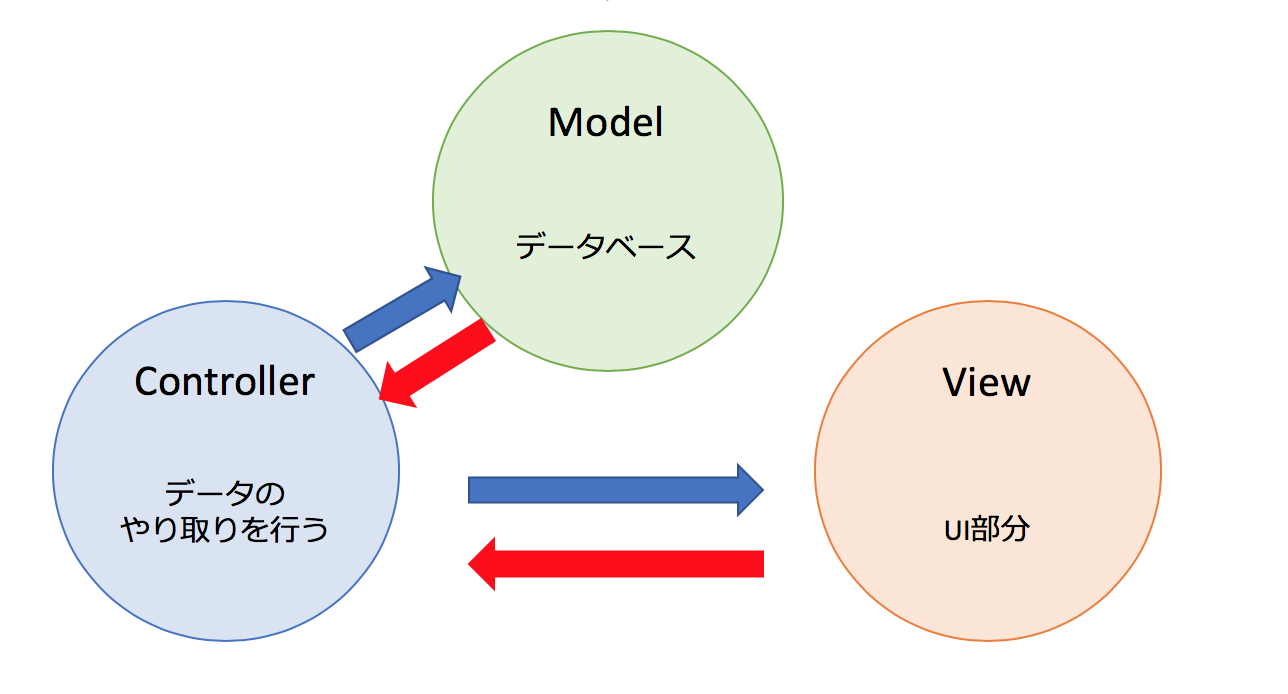
\includegraphics[clip,width=12.0cm,height=8.0cm]{img/mvc.png}
    \caption{MVCアーキテクチャ(いい感じの画像)}
    \label{fig:MVC}
  \end{center}
\end{figure}
